\documentclass{article}
\usepackage[utf8]{inputenc}
\usepackage{tikz}

\title{path-independence}
\author{ }
\date{January 2020}

\begin{document}

\maketitle

\section{Introduction}

Many systems can be understood as a a category, or a collection of sets, with some transformation functions between the sets- for example, in programming languages, type systems with coercion. If a graph is constructed with the sets as nodes and functions as edges between the nodes, then by construction the new graph has the property of "path independence", the idea being that each object has a unique representation in a given set in the system.

Much like conservative fields in physics, path independent graphs may arise in many systems. It might be useful to be able to perform some basic verification and ensure the graphs in question are indeed path independent. As a case study, gator, a domain specific graphics language that allows automatic conversion between geometric spaces internally creates a graph with he transformations between the spaces. 
In order for the compiler to give predictable results, gator requires that this space transformation graph be path independent.

Naively checking if all paths in a given graph are path independent could require a number of function equality checks as bad as factorial in the number of nodes, since a path consists of an ordering of nodes. As comparing function equalities can be expensive, we seek a more refined approach to verifying path independence, specifically over the course of online addition to a graph, as would be useful in cases like the gator compiler.


\section{Definitions}
\begin{enumerate}
    \item Path graph: A graph with vertices representing sets, and directed edges representing transformations functions between the sets. A path represents the composition of the transformation functions in the nodes.
    \item Conflicting paths: Paths with same source and destination node. (Note that in this definition of the term we don not require paths to actually disagree, but only have the potential to give different results).
    \item Path independence: The property that all conflicting paths in a graph are equal. Equality can be thought of as evaluated by some function equality checking oracle.
\end{enumerate}

\section{Identifying the set of new conflicting paths on addition of edge}

The naive approach to verifying path independence would be to compare all conflicting paths pairwise and thus ensure that there are no instances of violation of the property. Over the course of online addition of an edge, given that the graph before adding the edge was path independent, it would only be necessary to check conflicting pairs involving a new path that were created as a consequence of adding the new edge to the path.
To identify all such conflicting pairs, we present the \textit{two-flip tolerant path search}. This naive approach may be considered a baseline solution.

\subsection{Two flip tolerant path search}
In a normal directed graph path, only forward edges, i.e. edges that go outward from the current node, are considered. 
On the other hand, the \textit{two flip path} goes through up to three phases: in the first phase, only backward edges- pointing inward to the current node- are accepted. In the second phase, only forward edges are accepted, and in the third phase, again only backward edges are accepted. As a consequence, there is a node in the path for which both path edges are oriented outwards, that lies between the first and second phase. This will be referred to as the \textit{first flipping point}. Similarly, there is a \textit{second flipping point} between the second and third phase, for which both path edges point inwards.

Consider the situation where a new edge from source node S to sink T is being added to a graph.
A two flip tolerant path from S to T would correspond to a new pair of conflicting paths- flipping point 1 would be the source of both paths, and flipping point 2, the sink. The first path would correspond to the second phase of the flip tolerant path search, and the second path, involving the new edge, would correspond to composing the first phase of the two flip path, the new edge, and the third phase.

To present this idea diagrammatically, we represent path phases with arrows (note that these are the composition of many edges, not a single edge). The new edge is represented with a dashed arrow.


\begin{center}
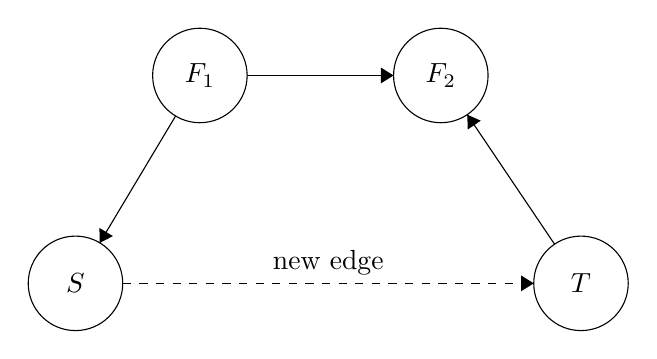
\begin{tikzpicture}[scale=0.2]
\tikzstyle{every node}+=[inner sep=0pt]
\draw [black] (18.1,-36.1) circle (3);
\draw (18.1,-36.1) node {$S$};
\draw [black] (50.2,-36.1) circle (3);
\draw (50.2,-36.1) node {$T$};
\draw [black] (26,-22.9) circle (3);
\draw (26,-22.9) node {$F_1$};
\draw [black] (41.3,-22.9) circle (3);
\draw (41.3,-22.9) node {$F_2$};
\draw [dashed] (21.1,-36.1) -- (47.2,-36.1);
\fill [black] (47.2,-36.1) -- (46.4,-35.6) -- (46.4,-36.6);
\draw (34.15,-35.6) node [above] {new edge};
\draw [black] (24.46,-25.47) -- (19.64,-33.53);
\fill [black] (19.64,-33.53) -- (20.48,-33.1) -- (19.62,-32.58);
\draw [black] (29,-22.9) -- (38.3,-22.9);
\fill [black] (38.3,-22.9) -- (37.5,-22.4) -- (37.5,-23.4);
\draw [black] (48.52,-33.61) -- (42.98,-25.39);
\fill [black] (42.98,-25.39) -- (43.01,-26.33) -- (43.84,-25.77);
\end{tikzpicture}
\end{center}
Here, (S, $F_1$, $F_2$, T) is a two flip tolerant path. ($F_1$, S, T, $F_2$) is a new path, created because of the addition of (S,T), that conflicts with ($F_1$, $F_2$).

The two flip tolerant path search returns the set of all paths between a given source and sink that have upto two flips (paths that omit one or more of the three phases are also accepted).

The \textit{path extraction algorithm} then transforms the output of the two flip path search to the set of new pairs of conflicting paths that arise in the graph due to its addition.

*= This excludes paths whose "area of difference" does not include the new edge since they should remain path independent. It also excludes paths that in their course contain cycles that exclude the new edge, since these paths must, again by path independence of the original graph, be equal to the path resulting from removing their cycles.

\paragraph{Path extraction algorithm}
The purpose of this algorithm is to derive the conflicting pairs that a given two-flip tolerant path corresponds to.

Let the new edge added to the graph be (S, T).
It has already been shown how each path corresponds to a conflicting pair in the case where a path has two flips. When a path has only the first flip (which is to say, the third phase of the path is missing), but not the second flip, sink node T can be treated as the sink of the two conflicting path, while the first flipping point remains the source. Similarly when only the second flipping point is present then it is the sink, and S is the source. Finally when no flipping points are present, there are two possibilities. 
Either the path is oriented from S to T, in which case the conflicting paths are simply the edge (S, T) and the entire flip-less path.
Or, the path is oriented from T to S. In this case, the conflicting paths are the identity on S (that implicitly exists) and the cycle obtained from composing the new edge with the path. The cycle conflicts with all other cycles starting from each node in the cycle. Notice that a single cycle can give rise to multiple conflicting pairs.


\paragraph{Theorem} The result of the two-flip tolerant path search from the source to the sink node of an edge that is to be newly added, followed with the path extraction algorithm has a one-to-one* correspondence to the set of new pairs of conflicting paths that arise in the graph due to its addition.

*= Same conditions as above.

\paragraph{Proof}

Every element in the output of the path extraction algorithm was by definition a conflicting pair.

It remains to show that every new conflicting pair corresponds to a two flip tolerant path. Let the common source be $F_1$ and common sink be $F_2$. 
Note that we are excluding pair where both paths include the new edge, since such paths are equal from $F_1$ to S because of the path independence of the original graph, identical from S to T, and again equal from T to $F_2$ because of original path independence. Being the composition of equal parts, these paths must always be equal.

Now, it is the case that only one path passes through (S, T), which we will name path 1. We construct a two flip tolerant path from S to T: phase 1 is the segment of path 1 from $F_1$ to S, phase 2 is path 2, and phase 3 is the segment of path 1 from T to $F_2$. It is possible that some of $F_1, F_2, S$ and $T$ coincide, in which case the corresponding segments between them disappear, and the resultant path has fewer than two flips.


\subsection{Implementation of two-flip tolerant path search}
A modified DFS with visited set also getting popped on backtrack (to get \textit{all} paths) and additionally, variables to maintain number of flips and flip state.

*Insert python code here*

\subsection{Implementation of path extraction}
 *Again, insert code*

\subsection{Verification using the new paths}
The algorithm returns pairs of conflicting paths. Verification is performed by composing edge functions to derive path functions, and then performing an equality check to verify if the path functions are equal.

If any of the paths don't check out then the graph, by definition, cannot be path independent. If all the paths do check out and the graph was originally path independent then the new graph is path independent, since new pairs have been verified and old pairs remain unchanged.

\subsection{Optimization of two-flip search}

The naive approach presented above identifies and verifies all conflicting pairs in the graph. However, because of the relationship between the various paths, there is some redundancy. It sometimes possible to conclude from verifying one pair, that a different pair must necessarily also be equal. We leverage such situations, since checking the equality of paths may be an expensive operation and an all-path search can have a bad worst-case run time. 

\subsubsection{Ordering on informativeness of paths}

Given a pair of two flip tolerant paths, we look at situations where there is a path between corresponding flipping points.
There are two cases.

\paragraph{Case 1} The arrows connecting flip points of path 1 to flip points of path 2 are in opposite directions.

\begin{center}
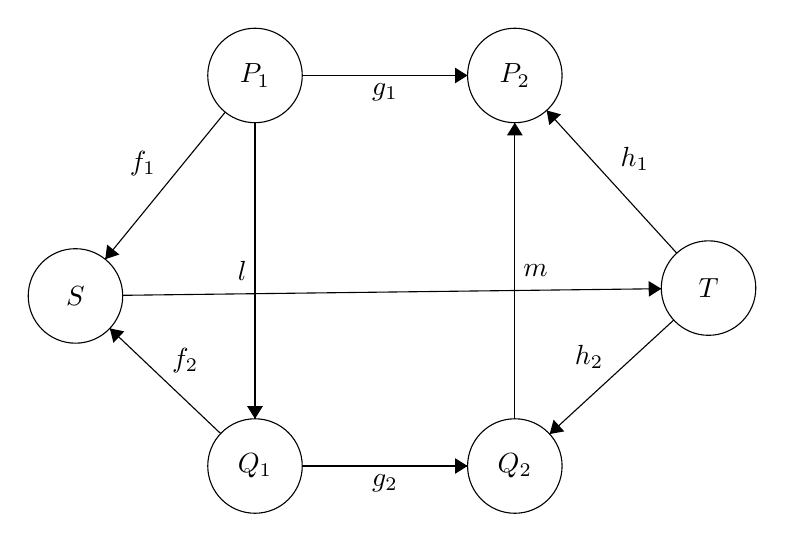
\begin{tikzpicture}[scale=0.2]
\tikzstyle{every node}+=[inner sep=0pt]
\draw [black] (16.6,-34.1) circle (3);
\draw (16.6,-34.1) node {$S$};
\draw [black] (56.8,-33.6) circle (3);
\draw (56.8,-33.6) node {$T$};
\draw [black] (28,-20.1) circle (3);
\draw (28,-20.1) node {$P_1$};
\draw [black] (44.5,-20.1) circle (3);
\draw (44.5,-20.1) node {$P_2$};
\draw [black] (28,-44.9) circle (3);
\draw (28,-44.9) node {$Q_1$};
\draw [black] (44.5,-44.9) circle (3);
\draw (44.5,-44.9) node {$Q_2$};
\draw [black] (31,-20.1) -- (41.5,-20.1);
\fill [black] (41.5,-20.1) -- (40.7,-19.6) -- (40.7,-20.6);
\draw (36.25,-20.6) node [below] {$g_1$};
\draw [black] (26.11,-22.43) -- (18.49,-31.77);
\fill [black] (18.49,-31.77) -- (19.39,-31.47) -- (18.61,-30.84);
\draw (21.74,-25.67) node [left] {$f_1$};
\draw [black] (25.82,-42.84) -- (18.78,-36.16);
\fill [black] (18.78,-36.16) -- (19.01,-37.08) -- (19.7,-36.35);
\draw (23.57,-39.02) node [above] {$f_2$};
\draw [black] (31,-44.9) -- (41.5,-44.9);
\fill [black] (41.5,-44.9) -- (40.7,-44.4) -- (40.7,-45.4);
\draw (36.25,-45.4) node [below] {$g_2$};
\draw [black] (54.59,-35.63) -- (46.71,-42.87);
\fill [black] (46.71,-42.87) -- (47.64,-42.7) -- (46.96,-41.96);
\draw (49.21,-38.76) node [above] {$h_2$};
\draw [black] (54.78,-31.38) -- (46.52,-22.32);
\fill [black] (46.52,-22.32) -- (46.69,-23.25) -- (47.43,-22.57);
\draw (51.19,-25.39) node [right] {$h_1$};
\draw [black] (28,-23.1) -- (28,-41.9);
\fill [black] (28,-41.9) -- (28.5,-41.1) -- (27.5,-41.1);
\draw (27.5,-32.5) node [left] {$l$};
\draw [black] (19.6,-34.06) -- (53.8,-33.64);
\fill [black] (53.8,-33.64) -- (52.99,-33.15) -- (53.01,-34.15);
\draw [black] (44.5,-41.9) -- (44.5,-23.1);
\fill [black] (44.5,-23.1) -- (44,-23.9) -- (45,-23.9);
\draw (45,-32.5) node [right] {$m$};
\end{tikzpicture}
\end{center}
Let Path$_1=f_1\circ g_1\circ h_1$ and Path$_2$=$f_2\circ g_2\circ h_2$. We choose Path$_2$.
\paragraph{Theorem} 
If conflicting paths $g_2 = f_2 \circ (S,T) \circ h_2$ then it must be that $g_1 = f_1 \circ (S,T) \circ h_1$.
\paragraph{Proof}
We use the fact that $f_1$=$l\circ f_2$ and $h_1$=$h_2 \circ m$.
\[g_2 = f_2 \circ (S,T) \circ h_2 \Rightarrow l \circ g_2 = l \circ f_2 \circ (S,T) \circ h_2 \Rightarrow l \circ g_2 \circ m = l \circ f_2 \circ (S,T) \circ h_2 \circ m \Rightarrow g_1 = f_1 \circ (S,T) \circ h_1\]

% Notice this ordering is like the subtyping rule for a function. What is the relationship?

Notice that this generalization will apply to situations where any of these paths are the identity, such as when the first flipping point of both paths is the same, or when there is no first flipping point- it is identical to S.

\paragraph{Case 2} The arrows connecting flip points of path 1 to flip points of path 2 are in the same directions.

\begin{center}
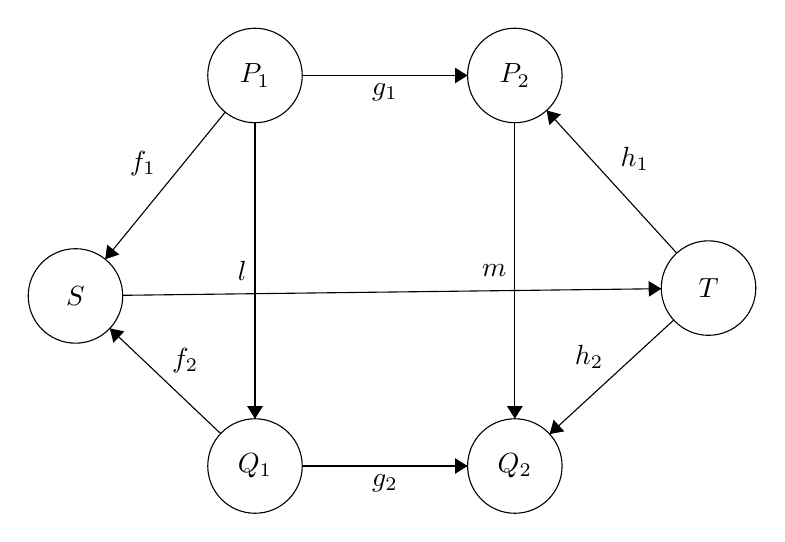
\begin{tikzpicture}[scale=0.2]
\tikzstyle{every node}+=[inner sep=0pt]
\draw [black] (16.6,-34.1) circle (3);
\draw (16.6,-34.1) node {$S$};
\draw [black] (56.8,-33.6) circle (3);
\draw (56.8,-33.6) node {$T$};
\draw [black] (28,-20.1) circle (3);
\draw (28,-20.1) node {$P_1$};
\draw [black] (44.5,-20.1) circle (3);
\draw (44.5,-20.1) node {$P_2$};
\draw [black] (28,-44.9) circle (3);
\draw (28,-44.9) node {$Q_1$};
\draw [black] (44.5,-44.9) circle (3);
\draw (44.5,-44.9) node {$Q_2$};
\draw [black] (31,-20.1) -- (41.5,-20.1);
\fill [black] (41.5,-20.1) -- (40.7,-19.6) -- (40.7,-20.6);
\draw (36.25,-20.6) node [below] {$g_1$};
\draw [black] (26.11,-22.43) -- (18.49,-31.77);
\fill [black] (18.49,-31.77) -- (19.39,-31.47) -- (18.61,-30.84);
\draw (21.74,-25.67) node [left] {$f_1$};
\draw [black] (25.82,-42.84) -- (18.78,-36.16);
\fill [black] (18.78,-36.16) -- (19.01,-37.08) -- (19.7,-36.35);
\draw (23.57,-39.02) node [above] {$f_2$};
\draw [black] (31,-44.9) -- (41.5,-44.9);
\fill [black] (41.5,-44.9) -- (40.7,-44.4) -- (40.7,-45.4);
\draw (36.25,-45.4) node [below] {$g_2$};
\draw [black] (54.59,-35.63) -- (46.71,-42.87);
\fill [black] (46.71,-42.87) -- (47.64,-42.7) -- (46.96,-41.96);
\draw (49.21,-38.76) node [above] {$h_2$};
\draw [black] (54.78,-31.38) -- (46.52,-22.32);
\fill [black] (46.52,-22.32) -- (46.69,-23.25) -- (47.43,-22.57);
\draw (51.19,-25.39) node [right] {$h_1$};
\draw [black] (28,-23.1) -- (28,-41.9);
\fill [black] (28,-41.9) -- (28.5,-41.1) -- (27.5,-41.1);
\draw (27.5,-32.5) node [left] {$l$};
\draw [black] (19.6,-34.06) -- (53.8,-33.64);
\fill [black] (53.8,-33.64) -- (52.99,-33.15) -- (53.01,-34.15);
\draw [black] (44.5,-23.1) -- (44.5,-41.9);
\fill [black] (44.5,-41.9) -- (45,-41.1) -- (44,-41.1);
\draw (44,-32.5) node [left] {$m$};
\end{tikzpicture}
\end{center}

In this case, nothing can be said. As a counterexample, let $P_1$ contain element a.
Suppose $g_1(a)=a_{g_1}$. Similarly, $l(a)=a_{l}$.
*TODO Write. Basically there can be a disagreement at $P_2$.*


\paragraph{Theorem} This reduction rule is the most general possible.
\paragraph{Proof} TODO write. Basically we create an axiom set where the only allowed action is composing with functions. This leads to only one inference rule to show implication between path equalities. We show that to derive p1>p2 using the inference rule some number of times, it is necessarily true that p1 and p2 have the relationship described in this case.

\section{Optimization}
We now present a polynomial time algorithm, that is based on the observation that all conflicting paths that have the same source and same sink, but do not include the new edge, must be equal because of path independence in the pre-existing graph. Therefore, it suffices to check for one path for a given source and sink, and it follows that all the rest will check out.

In terms of flip points, this is a special instance of case 1, where l and m are the identity.
\begin{center}
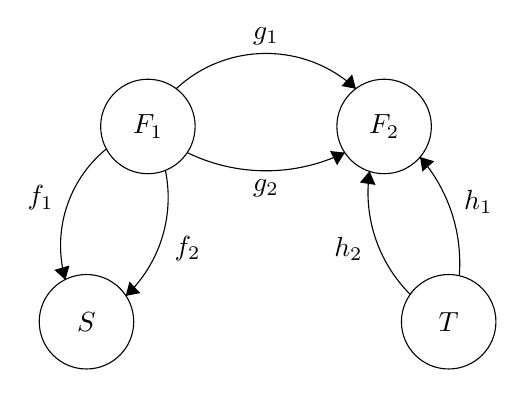
\begin{tikzpicture}[scale=0.2]
\tikzstyle{every node}+=[inner sep=0pt]
\draw [black] (25,-31.9) circle (3);
\draw (25,-31.9) node {$S$};
\draw [black] (48,-31.9) circle (3);
\draw (48,-31.9) node {$T$};
\draw [black] (28.9,-19.5) circle (3);
\draw (28.9,-19.5) node {$F_1$};
\draw [black] (43.9,-19.5) circle (3);
\draw (43.9,-19.5) node {$F_2$};
\draw [black] (30.687,-17.11) arc (132.96162:47.03838:8.383);
\fill [black] (42.11,-17.11) -- (41.87,-16.2) -- (41.19,-16.93);
\draw (36.4,-14.36) node [above] {$g_1$};
\draw [black] (41.409,-21.156) arc (-63.93383:-116.06617:11.399);
\fill [black] (41.41,-21.16) -- (40.47,-21.06) -- (40.91,-21.96);
\draw (36.4,-22.82) node [below] {$g_2$};
\draw [black] (23.657,-29.237) arc (-164.08097:-230.83744:7.929);
\fill [black] (23.66,-29.24) -- (23.92,-28.33) -- (22.96,-28.61);
\draw (22.95,-24.04) node [left] {$f_1$};
\draw [black] (30.007,-22.272) arc (11.75211:-46.67052:8.58);
\fill [black] (27.49,-30.26) -- (28.42,-30.08) -- (27.73,-29.35);
\draw (30.56,-27.24) node [right] {$f_2$};
\draw [black] (45.566,-30.169) arc (-134.8387:-188.56886:9.123);
\fill [black] (42.98,-22.34) -- (42.36,-23.06) -- (43.35,-23.21);
\draw (42.57,-27.26) node [left] {$h_2$};
\draw [black] (46.175,-21.439) arc (41.169:-4.57656:10.227);
\fill [black] (46.18,-21.44) -- (46.33,-22.37) -- (47.08,-21.71);
\draw (48.95,-24.27) node [right] {$h_1$};
\end{tikzpicture}
\end{center}

Thus, when flip points of the two paths are identical, they give the same information and it is safe to verify only one and discard the other. This means that after our path search gives us all two flip tolerant paths, we only need to verify one path for each unique choice of flip points, and can discard the rest of the paths.

In an N node graph, there are $^NP_2 = N(N-1)$ choices of flip points. Thus we can place a polynomial upper bound on the number of paths that actually need to be verified.

If we allow only Case 1 above as a reducing law, this bound is tight. 
This can be seen in the case where the graph contains 2N nodes besides S and T. We consider N of the nodes to be in group 1, and the other N to be in group 2. Every node in group 1 has a forward node to every node in group 2, as well as to S. T has a forward edge to every node in group 2. In this graph, on the addition of edge (S, T), $N^2$ paths need to be verified which is polynomial in 2N+2.

\subsection{Optimized Path Finding Algorithm}
We utilize this idea of selecting flip points to devise a polynomial time path search. This search does not return all flip tolerant paths, but rather, a path for every feasible choice of flipping point.

\begin{verbatim}
let (s,t) be the new edge.
The graph being used for path search does not contain (s,t).

# set of tuples storing conflicting pairs of paths
set_of_pairs = {}

for every node f_1 in the graph:
    for every node f_2 in the graph:
        try:
            find a path p_1 from f_1 to s.
            find a path p_2 from t to f_2.
            let path p= p_1 + (s,t) + p_2.
            find a path q from f_1 to f_2.
            add (p,q) to set_of_pairs    
        catch(path search failed):
            print('There is no conflicting pair from f_1 and f_2 such that
            one of the paths contains the new edge')

equality_check_verify(set_of_pairs)
            
\end{verbatim}

As observed earlier, the number of paths that this algorithm returns is asymptotically tight.

Also notice that if trying to optimize for path length (say, if composing functions is expensive) then "find any path" can be replaced with "find shortest path".

\subsection{Proof of correctness}

*TODO fill out*

- Ignoring cycle containing paths is ok

- No point in doing a pair unless exactly one has new edge

- Excepting the cases already dismissed, there is no conflicting pair such that its information is not covered by one of the paths in the final set (best way to write might be by cases).

\subsection{Minimal path set}
While the algorithm above eliminates a large amount of redundancy, there is still potential for reducing the number of path checks. This is something we would want to do in situations in which equality checking is very expensive. By paying a cost in run-time, it is possible to derive a minimal set of paths to verify.

We create a flip-point graph where each node represents a choice of flip point, so that there are $|V|^2$ nodes in all for every choice of flip point pair.
An algorithm is run on the original graph to mark ever node with the set of its predecessors and successors.
If node $n_1$ has a set of successors S and $n_2$ has a set of predecessors P then on the new flip-point graph we group together all the points in $S\times P$ in a set corresponding to the choice of adding $n_1, n_2$ to the minimal flipping point set. This is done for every node pair.
Now the set cover problem is solved on the flip-point graph, and a minimal flip point set is obtained.

The path finding algorithm is then performed with the minimal set as follows:

\begin{verbatim}
let (s,t) be the new edge.
The graph being used for path search does not contain (s,t).

# set of tuples storing conflicting pairs of paths
set_of_pairs = {}

for every node (f_1, f_2) in minimal_flipping_point_set:
    try:
        find a path p_1 from f_1 to s.
        find a path p_2 from t to f_2.
        let path p= p_1 + (s,t) + p_2.
        find a path q from f_1 to f_2.
        add (p,q) to set_of_pairs    
    catch(path search failed):
        print('There is no conflicting pair from f_1 and f_2 such that
        one of the paths contains the new edge')

equality_check_verify(set_of_pairs)
            
\end{verbatim}

\subsection{Proof of correctness}
TODO: Write. Basically just say you're applying the reduction rule.

\subsection{Proof of optimality}
TODO: Write. Really just use the definition of the set cover problem.

\section{Applications}

TODO. Gator and Scala?

\end{document}
